\newpage
\section{Praktischer Teil: Kalkulation eines neuen E-Bike-Modells in SAP-CO} \label{infos}
\subsection{Fallbeispiel}
Szenario: Global Bike möchte sein Produktportfolio um ein neues E-Bike-Modell erweitern. Für die Entscheidung über die Einführung und Preisgestaltung soll eine Kalkulation der voraussichtlichen Produktkosten erstellt werden.
 Um dieses Vorhaben in die Tat umzusetzen müssen folgende Schritte befolgt werden:
\\
\begin{figure}[H]
    \caption{Prozessverlauf Fallstudie}\label{fig:process}
    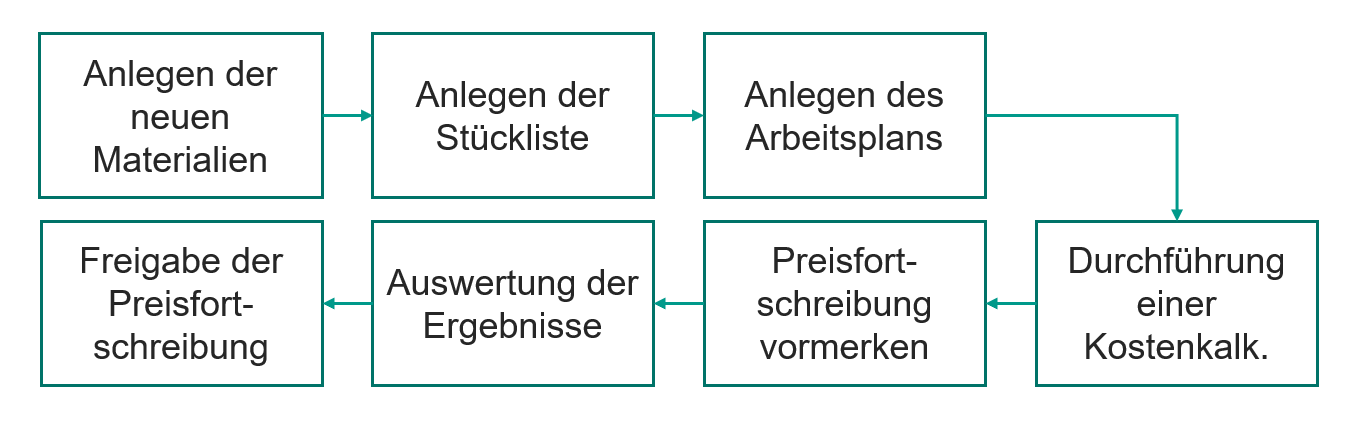
\includegraphics[width=0.9\textwidth]{ablauf}
    \\
    Quelle: Eigene Darstellung
\end{figure}
    
\begin{enumerate}
    \item \textbf{Anlegen der neuen Materialien}\\
    Das geplante E-Bike-Modell besteht aus verschiedenen Materialien. Die meisten dieser hat Global Bike bereits im System angelegt, da sie auch im Deluxe Touring Bike verbaut sind. Für das neue Modell müssen jedoch noch ein Elektromotor, ein Akku, und ein Ladekabel angelegt werden.
    \item \textbf{Anlegen der Stückliste}\\
    Die Stückliste enthält alle Materialien, die für die Produktion des E-Bikes benötigt werden. Sie gibt außerdem Auskunft darüber in welcher Menge die Materialien benötigt werden.
    \item \textbf{Anlegen des Arbeitsplans}\\
    Der Arbeitsplan enthält alle Arbeitsschritte, die für die Produktion des E-Bikes notwendig sind. Er gibt außerdem Auskunft darüber, wie lange die einzelnen Arbeitsschritte dauern und welche Ressourcen benötigt werden.
    \item \textbf{Durchführung der Kostenkalkulation}\\
    Die Kostenkalkulation gibt Auskunft darüber, wie hoch die voraussichtlichen Produktionskosten für das E-Bike sind. Sie setzt sich aus den Materialkosten, den Fertigungskosten und den Gemeinkosten zusammen. Dinge wie Vermarktungskosten oder Gewinnmarge sind hier noch nicht enthalten.
    \item \textbf{Vormerken der Preisvorschreibung}\\
    Der kalkulierte Preis wird zunächst als Vorschlag für die Preisvorschreibung vorgemerkt und in den Materialstammsatz übertragen. Dies ist der erste von zwei Schritten aus welchen die Preisfortschreibung besteht.
    \item \textbf{Auswertung der Ergebnisse}\\
    Die Ergebnisse der Kostenkalkulation werden Analysiert. Dabei wird geprüft, ob die kalkulierten Kosten in etwa den erwarteten Kosten entsprechen und ob auf dieser Basis ein auf dem Markt konkurrenzfähiger Preis festgelegt werden kann.
    \item \textbf{Freigabe der Preisvorschreibung}\\
    Nachdem die Erbegbnisse der Kostenkalkulation Analysiert wurden, und die Entscheidung positiv ausgefallen ist wird die Preisvorschreibung freigegeben. Dies ist der zweite Schritt aus welchen die Preisfortschreibung besteht und der Preis wird hier endgültig festgelegt.
\end{enumerate}
    
\subsection{Dokumentation und Erklärung}
Im folgenden werden die einzelnen Schritte des Prozesses anhand ausgewählter Grafiken genauer erläutert und dokumentiert. Für die Durchführung der Schritte wurde SAP-Fiori verwendet.
\subsubsection{Anlegen der neuen Materialien}
Da noch nicht alle benötigten Bauteile für das neue E-Bike-Modell, sowie das E-Bike selbst im System vohanden sind, müssen diese zunächst angelegt werden.
 Navigieren Sie dazu unter dem Reiter \textit{Controlling} zur Karte \textit{Material anlegen} und wählen Sie diese aus. Nun öffnet sich das Fenster 
 \textit{Material anlegen (Einstieg)}. Hier müssen Sie nun bei \textit{Material} das Material eingeben, welches Sie anlegen wollen. Da wir mit dem Elektromotor für das E-Bike starten,
 müssen Sie das Material \textit{EBEN1201} abgeben. Weiterhin müssen Sie nun noch die passende
 \textit{Branche}, im Beispiel \textit{"Maschienenbau"}, und eine passende \textit{Materialart}, im Beispiel \textit{"Rohstoff"}, auswählen. Sollten sie schon ein Material im System haben, 
 welches sich als Vorlage für das neue Material anbietet können Sie dieses noch im Bereich \textit{"Kopieren aus..."} bei \textit{"Material"} eingeben.
\begin{figure}[H]
    \caption{Anlegen des Materials}\label{fig:material}
    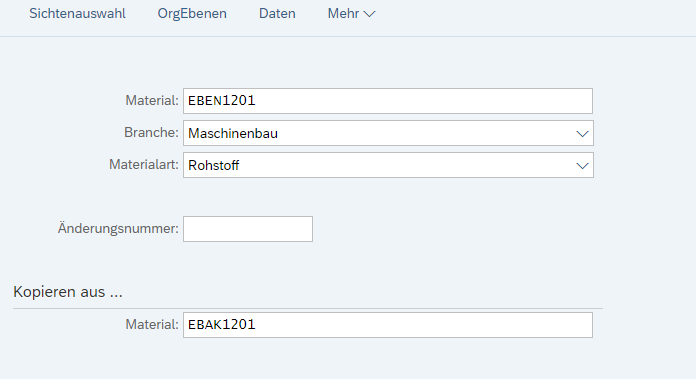
\includegraphics[width=0.9\textwidth]{Material Anlegen}
    \\
    Quelle: Eigene Darstellung
\end{figure}
Wenn Sie alles richtig eingegeben haben, können Sie nun auf \textit{Weiter} klicken und müssen in einem neuen Fenster mit Titel \textit{Sichtenauswahl} die Sichten
 \textit{Grunddaten 1}, \textit{Grunddaten 2}, \textit{Disposition 1} und \textit{Buchhaltung 1} selektieren. Wählen Sie, nachdem Sie die Sichten gewählt haben, den grünen Haken um fortzufahren.
\begin{figure}[H]
    \caption{Sichtenauswahl}\label{fig:sichtenauswahl}
    \includegraphics[width=0.9\textwidth]{Sichtenauswahl}
    \\
    Quelle: Eigene Darstellung
\end{figure}
Im nächsten Fenster müssen Sie nun noch das Werk angeben. Für das Beispiel wählen wir das Werk in Dallas namens \textit{DL00}. Wählen Sie nun den grünen Haken um fortzufahren.
\begin{figure}[H]
    \caption{Werk auswählen}\label{fig:werk}
    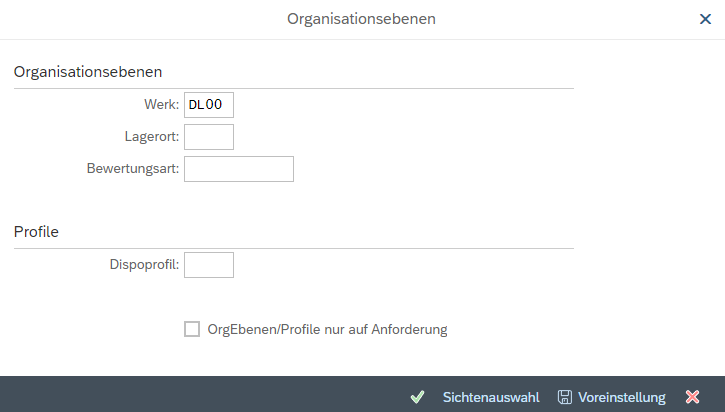
\includegraphics[width=0.9\textwidth]{Werk}
    \\
    Quelle: Eigene Darstellung
\end{figure}
In dem nun folgenden Fenster können Sie nun die passenden Daten für das Material eingeben. Geben Sie in der Sicht \textit{Grunddaten 1} in das Feld \textit{Bezeichnung}
 den Namen des Materials, also \textit{E-Bike Motor} ein, und wählen Sie als Basismengeneinheit \textit{ST} für Stück aus.
\begin{figure}[H]
    \caption{Grunddaten 1 - Bezeichnung und Allgemeine Daten}\label{fig:grunddaten1.1}
    \includegraphics[width=0.9\textwidth]{Grunddaten1.1}
    \\
    Quelle: Eigene Darstellung
\end{figure}
 
 Geben Sie weiterhin für \textit{Bruttogewicht} und \textit{Nettogewicht} 1000 und für die \textit{Gewichtseinheit} G ein.

\begin{figure}[H]
    \caption{Grunddaten 1 - Abmessungen}\label{fig:grunddaten1.2}
    \includegraphics[width=0.9\textwidth]{Grunddaten1.2}
    \\
    Quelle: Eigene Darstellung
\end{figure}
